\chapter{Design}\label{design_ch}
This Chapter will describe the design for the proposed solution, in the end a list of functionalities and requirements will be created which will be the basic for the implementation in the next Chapter.


\section{Overview}
The solution that has been proposed is to use the gestures defined in Figure \ref{pitch} and \ref{roll} instead of using a VAS. The orientation for each gesture should be translated to a value on a scale from zero to ten. To achieve this a wristband equipped with an IMU and a button will be used, the user will use one of the gestures and the press of the button to input the desired value. In order to view the data the wristband will be accompanied by a smartphone app. The companion app will display the logged data and offer the possibility to export it to a data file. This design is illustrated in Figure \ref{design_overview}.

Since the main focus of this report is to compare the gesture based input method to a VAS, the approach to the design of the companion app will be to create a Minimum Viable Product (MVP)\cite{mvp}. This means that it will focus a minimal set of features, just enough to be use able, like vise the user interface (UI) will be kept simple.

\begin{figure}[h]
    \centering
    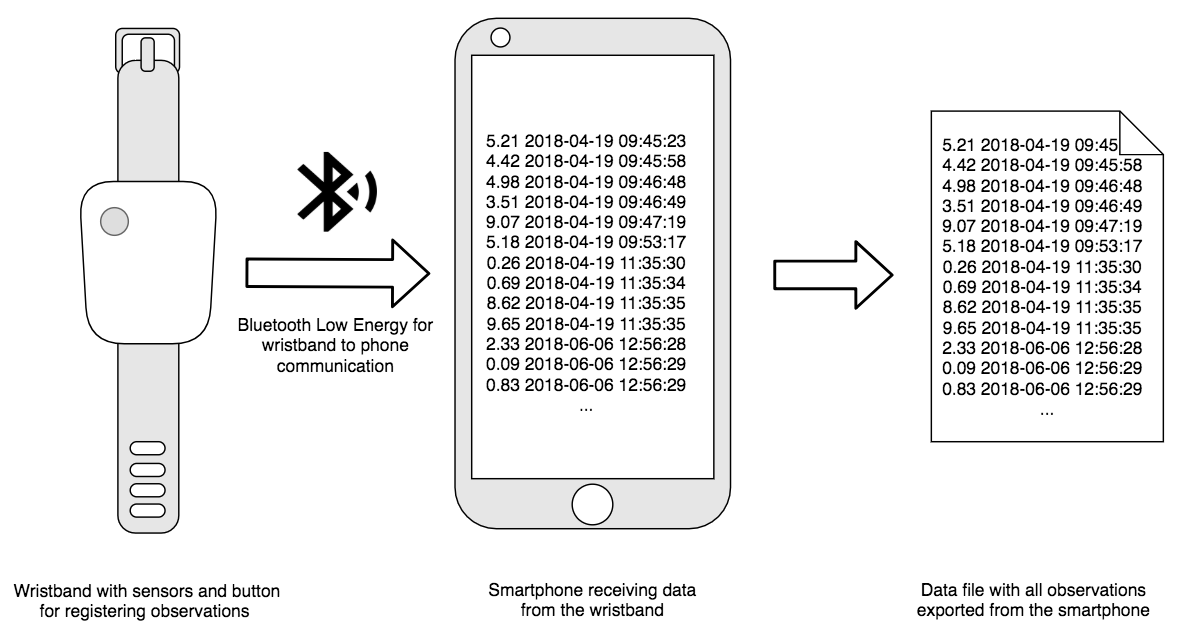
\includegraphics[width=1\textwidth]{figures/design_overview.png}
    \caption{Wristband device with sensors and a button for registering observation. Smartphone to import, display and export the data}
    \label{design_overview}
\end{figure}

\section{From Gesture to Value}
In order to convert a gesture to a value on a scale we must first define said gestures and then create function to map their measurement to the preferred scale. We shall start by defining the gestures based on the orientation of the arm.

\subsection{Orientation of the Arm}
With the orientation defined as the rotation of the three axis, we need to translate this into movement of the arm. In Figure \ref{pitch}, \ref{roll} and \ref{yaw} the movement to adjust pitch, roll and yaw is described.

Pitch is changed by rotating the arm around the elbow, resulting in the lower arm being raised/lowered. The angle between the lower arm and table (horizontal plane) is then the measurement for this rotation.

\begin{figure}[h!]
    \centering
    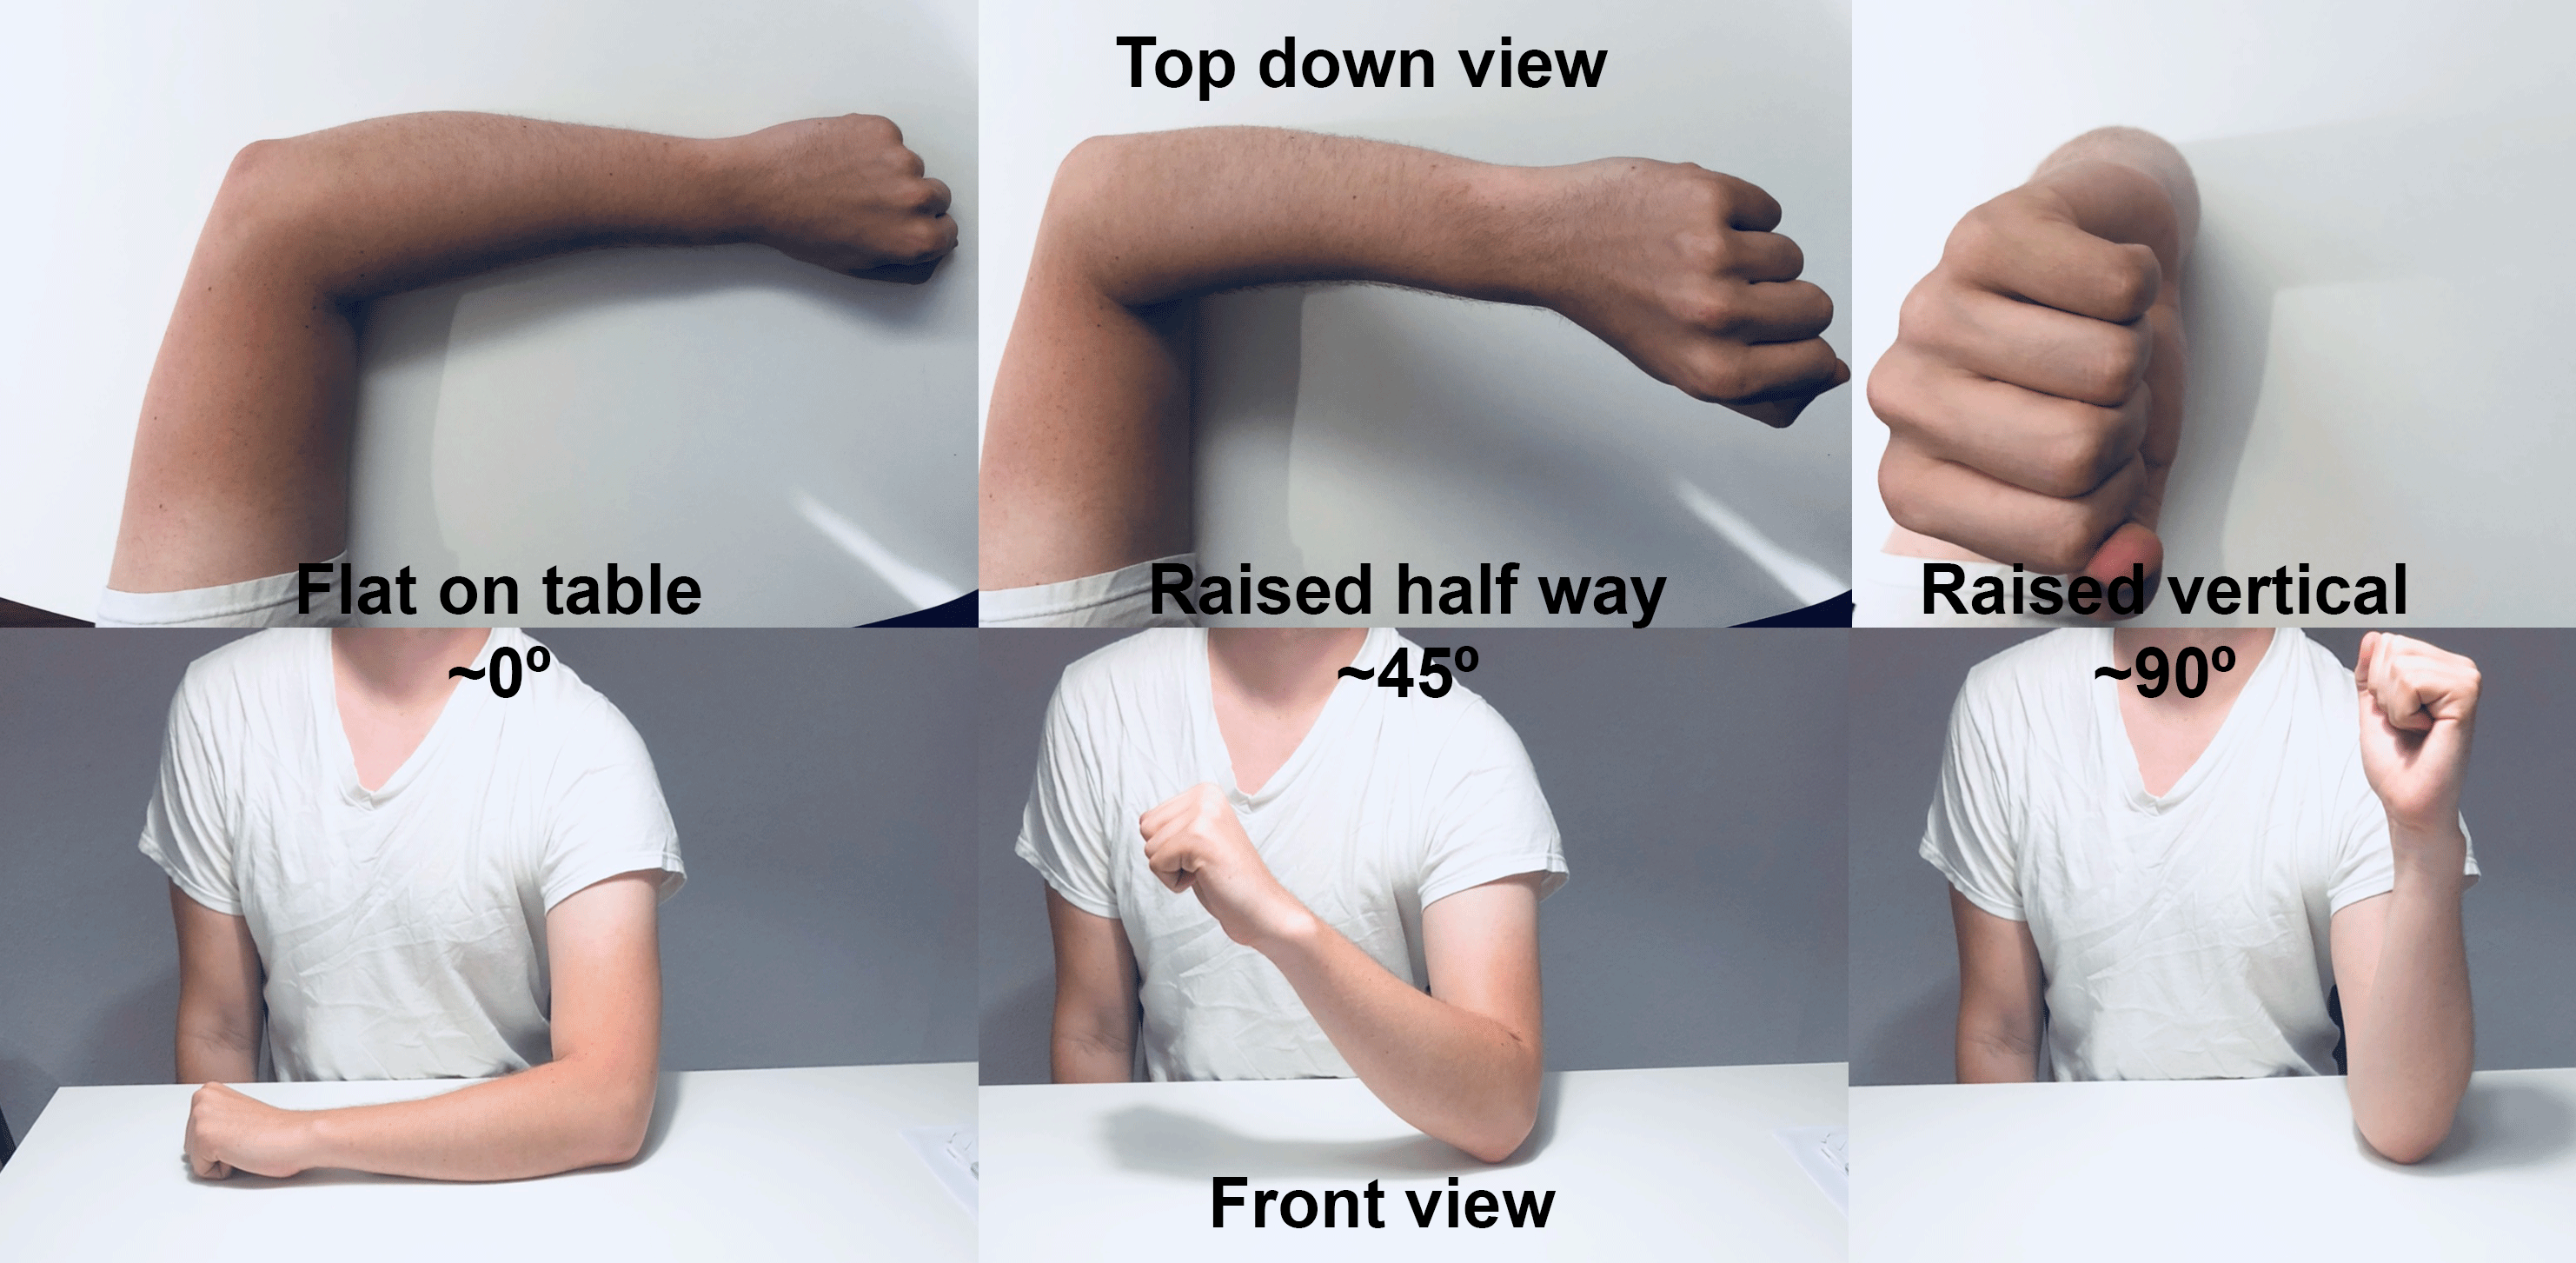
\includegraphics[width=1\textwidth]{figures/pitch.png}
    \caption{The movement for adjusting \underline{pitch} by rotating the arm around the elbow}
    \label{pitch}
\end{figure}

Roll is changed by rotating the wrist/lower arm, the angle between the back of the hand and table is then the measurement for this rotation.

\begin{figure}[h!]
    \centering
    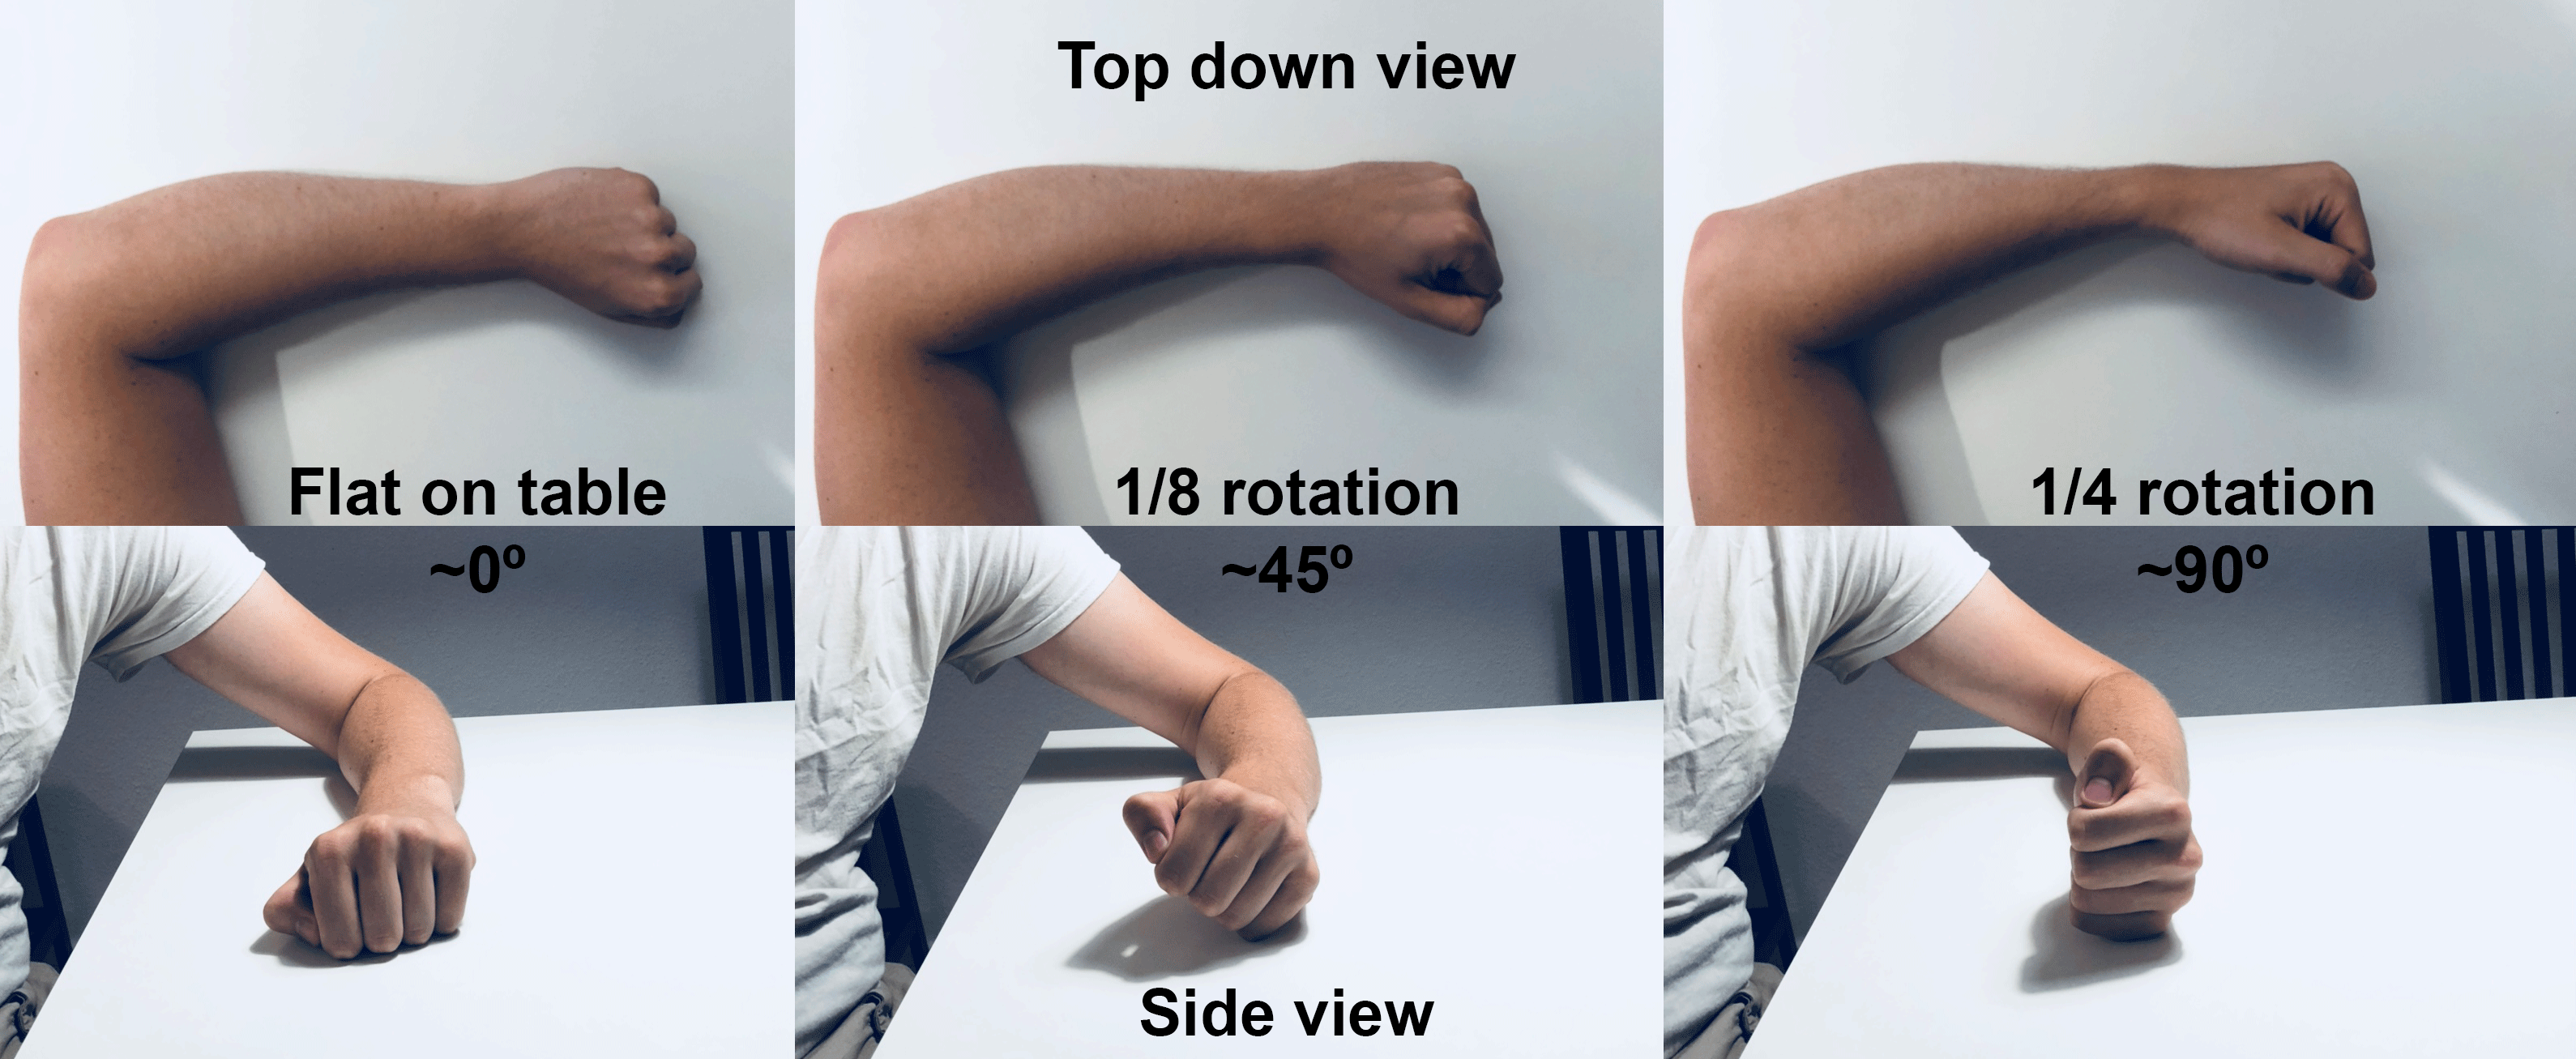
\includegraphics[width=1\textwidth]{figures/roll.png}
    \caption{The movement for adjusting \underline{roll} by rotating the wrist/lower arm}
    \label{roll}
\end{figure}

Yaw is changed by bending the lower arm the elbow, keeping it level with the table, thus changing the direction of the lower arm. The angle of direction is then the measurement for this rotation.

\begin{figure}[h!]
    \centering
    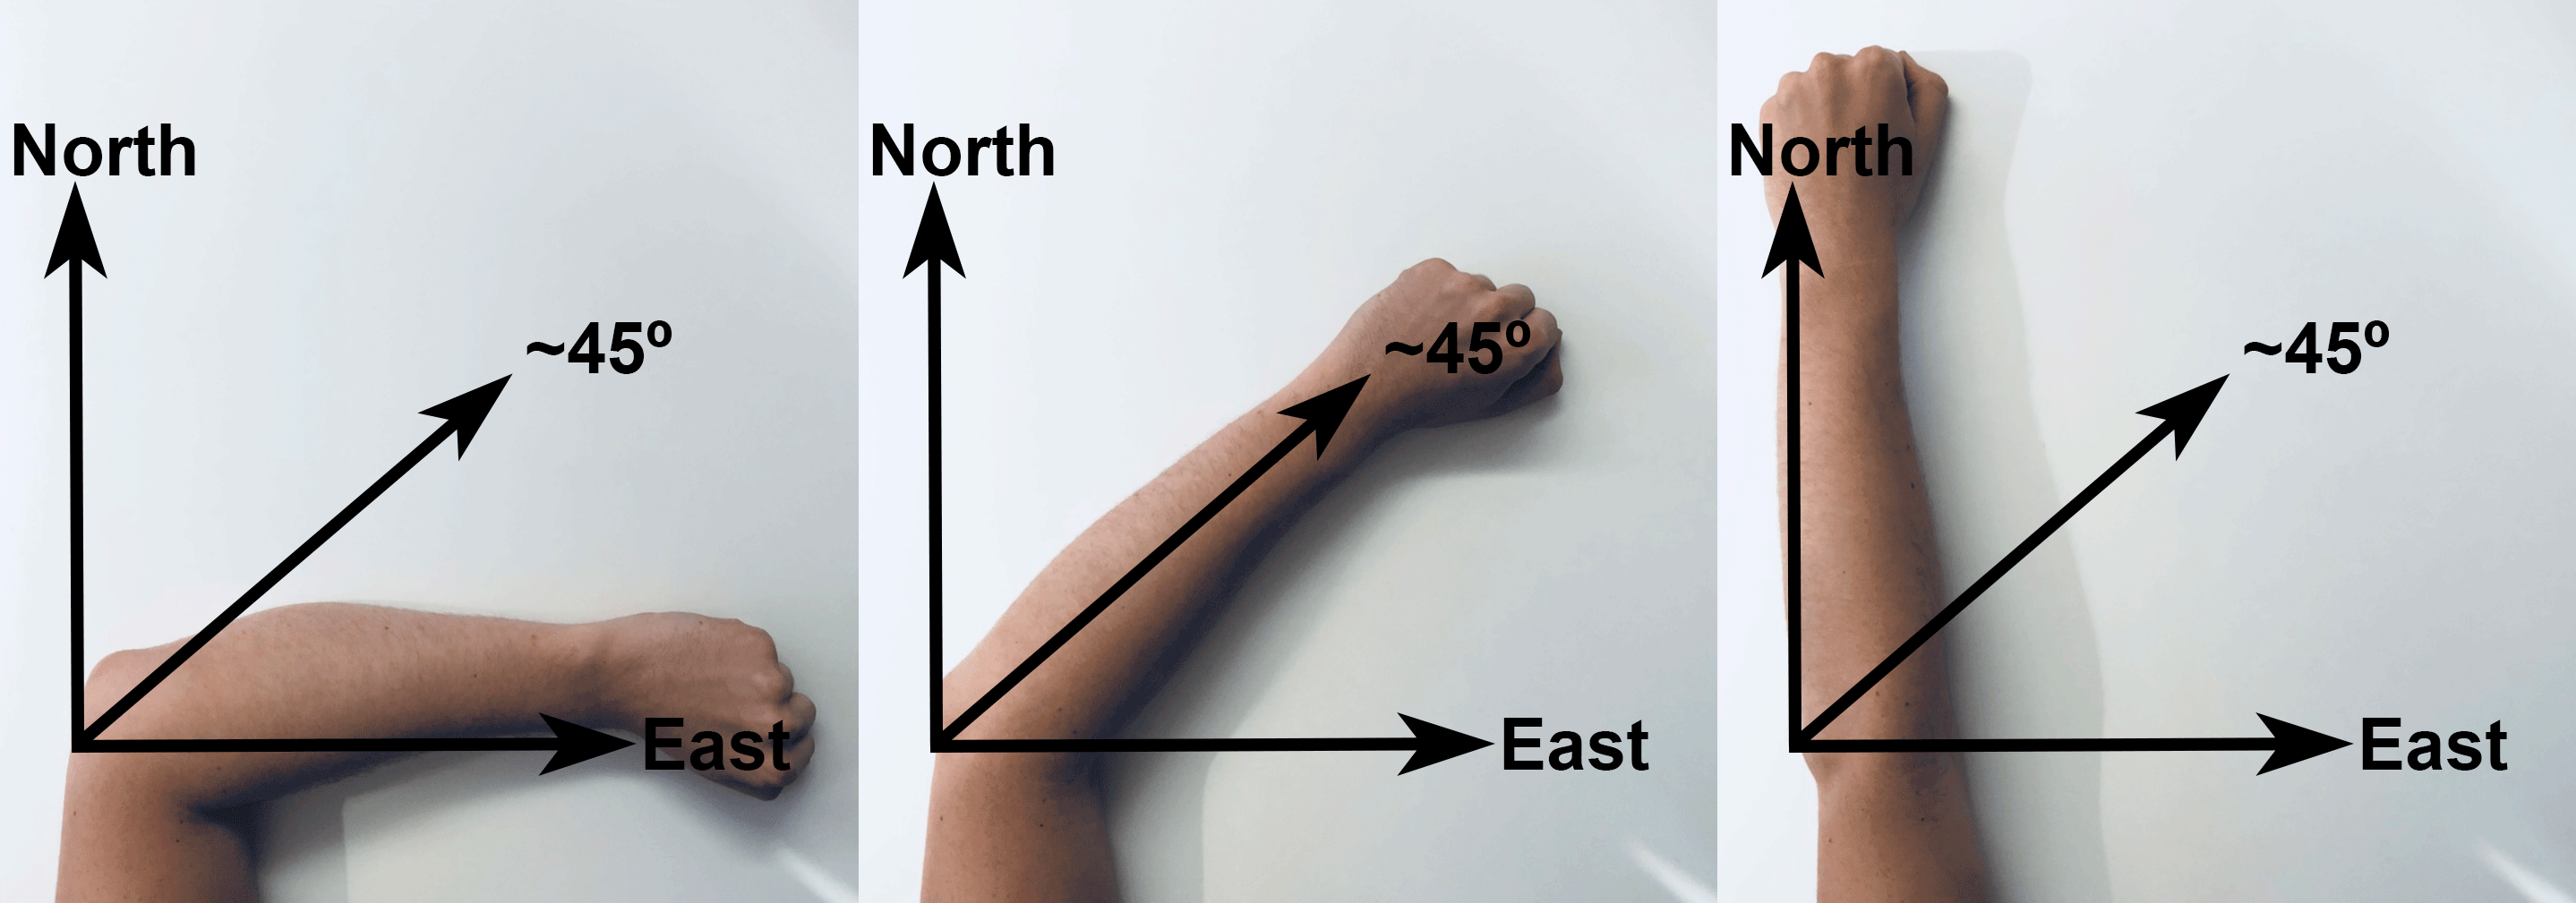
\includegraphics[width=1\textwidth]{figures/yaw.png}
    \caption{The movement for adjusting \underline{yaw} by rotating the lower arm around the elbow (note the arm is flat/horizontal on the table)}
    \label{yaw}
\end{figure}

Of course all three rotation can be achieved in other ways, for example yaw can be changed by turning the entire body to face another directions. But for the purpose of this thesis we look at these motions because they are done in front of one self, can be executed both while sitting at a table (for best reference) or while standing, and for all these motions the body itself also is a reference point, where turning your entire body would require another reference point to make sense of the scale.

\subsection{Problems with Yaw}
As described when measuring absolute orientation, then the magnetic north is used as the calibration point, meaning that 0º yaw will be pointing north, 90º pointing east and so on. Both pitch and roll is relative to the ground (horizontal plane), therefore no matter the yaw orientation you can get an absolute reading based on one point within the arm movement described earlier, e.g. you can rotate your wrist to a desired angle and take one measurement and know the orientation in that axis. This can't be done for yaw, it would require that you either first align yourself to a specific direction (north for example), and then bend the lower arm out in front to the desired angle, or it requires two measurement (one in the starting position, and one in the desired position) in order to calculate the difference, and achieve the desired angle. For this reason using the yaw orientation will not be investigated further, since it would introduce a higher burden for the user.

\subsection{Mapping Euler Angles to a 0-10 Scale}
We have now defined the two gestures as seen in Figure \ref{roll} and \ref{pitch}, we shall refer to them as wrist and arm gesture. We will assume that performing both gestures will have a linear relation between the movement and the Euler angle measured. As mentioned the roll angle will always be between -90º and 90º depending if the orientation clock or counter clock wise compared to 0º (horizontal). To map the values to a 0-10 scale the absolute value is divided by 9, e.g 90º and -90º will become 10, 45º and -45º will become 5, 25º and -25º will become 2.7778 etc. Mathematically this can be expressed with the function seen in Equation \ref{eq_roll} where \emph{sv} is the scaled value from 0-10 and \emph{ra} is the Euler angle for the roll axis.

\begin{eqfloat}
\begin{equation}
sv\left ( ra \right ) = \frac{abs\left (ra\right )}{9}
\label{eq:linear}
\end{equation}
\caption{Mapping roll angle (ra) to scaled value (sv)}
\label{eq_roll}
\end{eqfloat}

A consequence of this mapping is that if the wristband is turned pass the vertical position the scaled value will begin to decrease. This means that the user won't achieve a 10 rating simply by turning the wrist way beyond the vertical position. A different solution could be made to detect when the wristband pass the vertical position and set the scaled value at 10. It can be debated as to which solution is the greater, but by letting the scaled value decrease will force the user to get a better sense of the scale and won't allow \say{lazy} inputs.

Mapping the pitch angle needs to take into account that the roll value will be between -180º and 180º. The solution is to create a function that maps the value differently depending if the absolute pitch angle is greater than 90, basically first mapping the -180º to 180º range down to a -90º to 90º degree range, and then mapping it to the scaled value. The function in Equation \ref{eq_pitch} will express this where \emph{sv} is the scaled value from 0-10 and \emph{pa} is the Euler angle for the pitch axis.

\begin{eqfloat}
\begin{equation}
sv\left ( pa \right ) = \left\{\begin{matrix}
\frac{90-\left ( abs\left ( pa \right )-90 \right )}{9} & if\ abs(pa) > 90 \\ 
\frac{abs\left ( pa \right )}{9} & otherwise
\end{matrix}\right.
\label{eq:linear}
\end{equation}
\caption{Mapping pitch angle (pa) to scaled value (sv)}
\label{eq_pitch}
\end{eqfloat}


\section{Functionalities and Requirements}\label{requirements}
With the general outline for the wristband and companion app laid out, we can create a list of functionalities and requirements that shall be implemented in order to create a MVP.

\begin{itemize}
    \item \textbf{Log data:} The user should be able to log observation using the wristband, this should be possible to do independently from the companion app
    \item \textbf{Import data:} The companion app shall import the logged data from the wristband
    \item \textbf{Display data:} The companion app shall display the logged data (scaled value and time stamp)
    \item \textbf{Export data:} The companion app shall be able to export the logged data to a data file for further investigation
	\item \textbf{Simple solution:} It should be simple and easy to perform all of the above actions.
\end{itemize}